\documentclass[sigconf,review=false,anonymous=true]{acmart}

\usepackage{booktabs} % For formal tables
\usepackage{balance}

\usepackage[toc,page]{appendix}


% remove next three lines for CRC
% Removes citation information below abstract
\settopmatter{printacmref=false} 
% removes footnote with conference information in first column
\renewcommand\footnotetextcopyrightpermission[1]{} 
% removes running headers
\pagestyle{plain} 


% Copyright
%\setcopyright{none}
%\setcopyright{acmcopyright}
%\setcopyright{acmlicensed}
% \setcopyright{rightsretained}
%\setcopyright{usgov}
%\setcopyright{usgovmixed}
%\setcopyright{cagov}
%\setcopyright{cagovmixed}
\usepackage{dirtytalk}
\usepackage{enumitem}
\setlist{nolistsep}
\usepackage[utf8]{inputenc}
\usepackage{color}
\usepackage{graphicx}
\usepackage{grffile}
\usepackage{transparent}
\usepackage{pgfplotstable}
\usepackage[linesnumbered,ruled]{algorithm2e}
\usepackage{listings}
\usepackage{listings-golang}
\lstset{
  basicstyle=\ttfamily,
  columns=fullflexible,
  numbers=left,
  numbersep=5pt,
  showstringspaces=false, 
  stringstyle=\color{red},
  language=Golang,
  frame=single,
  keywordstyle=\color{blue},
  tabsize=2,
  breaklines=true,
  postbreak=\mbox{\textcolor{red},{$\hookrightarrow$}\space},
}
\usepackage{soul}
\colorlet{soulgreen}{green!30}
\definecolor{light-gray}{gray}{0.90}
\newcommand\mycommfont[1]{\footnotesize\ttfamily\textcolor{blue}{#1}}
\SetCommentSty{mycommfont}
\newcommand{\projectname}{Finch}

% for commenting and making it visible in the pdf (easy to hide after)
\newboolean{hidecomments}
\setboolean{hidecomments}{false}
%\nochangebars
\ifthenelse{\boolean{hidecomments}}
{\newcommand{\cb}[2]{}}
{\newcommand{\cb}[2]{
    \fbox{\bfseries\sffamily\scriptsize#1}
    {\sf\small$\blacktriangleright$ %$\RHD$
      {#2} $\blacktriangleleft$}}} %\LHD$}}}%
\newcommand\ra[1]{\cb{RA}{\textcolor{red}{#1}}}
\newcommand\rth[1]{\cb{RH}{\textcolor{green}{#1}}}

\newcommand{\inlquo}[1]{``\textit{#1}''}
\newcommand{\inlquoP}[2]{``\textit{#1}'' \textit{(#2)}}
\newcommand{\quo}[2]{\\[0.1cm]\noindent ``\textit{#1}'' \textit{(#2)}\vspace*{0.1cm}}
\newcommand{\quoWSp}[2]{\noindent ``\textit{#1}'' \textit{(#2)}}



% DOI
%\acmDOI{10.475/123_4}
% ISBN
%\acmISBN{123-4567-24-567/08/06}

%Conference
%\acmConference[WOODSTOCK'97]{ACM Woodstock conference}{July 1997}{El Paso, Texas USA} 
%\acmYear{1997}
%\copyrightyear{2016}


%\acmArticle{4}
%\acmPrice{15.00}

% These commands are optional
%\acmBooktitle{Transactions of the ACM Woodstock conference}
%\editor{Rodrigo Araújo}
%\editor{Reid Holmes}


\begin{document}
\title{Enabling Configuration Self-Adaptation\\ Using Machine Learning}

\author{Rodrigo Araújo}
%\orcid{1234-5678-9012}
\affiliation{%
  \department{Department of Computer Science}
  \institution{University of British Columbia}
  \city{Vancouver, Canada} 
}
\email{rodarauj@cs.ubc.ca}

\author{Reid Holmes}
\affiliation{%
  \department{Department of Computer Science}
  \institution{University of British Columbia}
  \city{Vancouver, Canada} 
}
\email{rtholmes@cs.ubc.ca}

% The default list of authors is too long for headers.
% \renewcommand{\shortauthors}{B. Trovato et al.}


\begin{abstract}
Due to advancements in distributed systems and the increasing industrial demands placed on these systems, distributed systems are comprised of multiple complex components (e.g databases and their replication infrastructure, caching components, proxies, and load balancers) each of which have their own complex configuration parameters that enable them to be tuned for given runtime requirements. Software  Engineers must manually tinker with many of these configuration parameters that change the behaviour and/or structure of the system in order to achieve their system requirements. In many cases, static configuration settings might not meet certain demands in a given context and ad hoc modifications of these configuration parameters can trigger unexpected behaviours, which can have negative effects on the quality of the overall system.

In this work, we show the design and analysis of Finch; a tool that injects a machine learning based MAPE-K feedback loop to existing systems to automate how these configuration parameters are set. Finch configures and optimizes the system to meet service-level agreements in uncertain workloads and usage patterns. Rather than changing the core infrastructure of a system to fit the feedback loop, Finch asks the user to perform a small set of actions: instrumenting the code and configuration parameters, defining service-level objectives and agreements, and enabling programmatic changes to these configurations. As a result, Finch learns how to dynamically configure the system at runtime to self-adapt to its dynamic workloads.

We show how Finch can replace the trial-and-error engineering effort that otherwise would be spent manually optimizing a system's wide array of configuration parameters with an automated self-adaptive system.

\end{abstract}

%
% The code below should be generated by the tool at
% http://dl.acm.org/ccs.cfm
% Please copy and paste the code instead of the example below. 
%
%\begin{CCSXML}
%<ccs2012>
% <concept>
%  <concept_id>10010520.10010553.10010562</concept_id>
%  <concept_desc>TBD~TBD</concept_desc>
%  <concept_significance>500</concept_significance>
% </concept>
%</ccs2012>  
%\end{CCSXML}
%\ccsdesc[500]{TBD~TBD}


%\keywords{ACM proceedings, \LaTeX, text tagging}

\maketitle

%!TEX root = main.tex

\section{Introduction}
\label{sec:introduction}

The industrial adoption of microservices has led to increasingly complex configuration schemes that are manually fine-tuned by engineers. Ganek and Corbi discussed the need for autonomic computing to handle the complexity of managing software systems~\cite{ganek_dawning_2003}. They noted that managing complex systems has become too costly, prone to error, and labour-intensive because pressured engineers make mistakes, increasing the potential of system outages with a concurrent impact on business. This has driven many researchers to study self-adaptive systems (e.g., \cite{porter_rex:_2016, andrew_pavlo_self-driving_2017, salehie_self-adaptive_2009, ganapathi_predicting_2009, herbst_self-adaptive_2014, faniyi_architecting_2014}); however, the software industry still lacks practical tools to provide self-adaptation mechanisms to their systems\rth{should we soften this to be about self-adaptive system configurations? This would better match what came before and comes after.}. Thus, most system configuration and tuning is performed manually, often at runtime, which is known to be a very time consuming and risky practice \cite{ganek_dawning_2003, using_prob_reasoning_automate_software_tuning, de_lemos_software_2013}.

In this work we present \projectname{}, a tool that enables engineers to integrate self-adaptation mechanisms into their systems. \projectname{} delegates the configuration and tuning of a system to a learned model, rather than requiring engineers to perform these operations manually or through manually tuned heuristics.

Building self-adaptive systems is a major engineering challenge \cite{brun_engineering_2009}. \projectname{}'s proposal is to enable self-adaptation by giving the user the ability to inject the main components of a self-adaptive mechanism into an existing target system in a loosely-coupled fashion.

One of our main goals is to provide self-adaptive configuration support with minimal engineer effort. \projectname{} uses ideas from system observability, machine learning, and control theory to automatically asses the system's environment, predict the impact of changes that could potentially improve the system, and make these changes automatically.

Our approach consists of providing mechanisms for injecting a control loop into an existing target system through an API for collecting relevant system metrics and configurations as the system executes. We map Service Level Agreements (SLAs) to a subset of these metrics, feed them into a machine learning component that is concurrently relearning the model while analyzing current event data which then predicts optimal configurations for the system for its given load. As a result, \projectname{} provides adaptation plans that can be both \emph{automatically executed}, allowing the system to have self-adaptive capabilities, and \emph{interpretable}, allowing engineers to understand the impact of a change in the configuration space before it is deployed.

\projectname{} not only provides reactive adaptations---adaptations that happen only when a constraint is violated---but also provides predictive adaptation plans that can be executed before a violation occurs. This is achieved by predicting the context of the observed system.

Our main contributions are:

\begin{itemize}
  \item A methodology for assisting the development and evolution of self-adaptive configuration systems, regardless of the presence of self-adaptability in the system's foundations. Such methodology is encapsulated in \projectname{}.
  \item Demonstrating how minimal changes to the system can support this approach, and how SLAs/SLOs can be modelled and mapped to optimization objectives. %These tasks being the development cost incurred by the engineers.
  \item Presenting a case study that shows how a system's response time, throughput, and usage were improved by $A\%$, $B\%$, and $C\%$ respectively after the integration of \projectname{}.
\end{itemize}

Section 2 discusses past research in the space of self-adaptive systems and provides fundamental background for our approach. Section 3 outlines our approach, explaining the blend of ideas from different fields that lead to its principle design decisions. Section 4 describes \toolname{} and its implementation. Section 5 presents our case study, followed by a discussion and future directions in Section 6.

%
% here we reorganize these characteristics into the following terminology:

% \begin{itemize}
%   \item \textbf{Self-Awareness}: an autonomic system needs to know itself;
%   \item \textbf{Self-configuring}: an autonomic system must configure and reconfigure itself under varying and unpredictable conditions;
%   \item \textbf{Self-optimization}: an autonomic system never settles for the status quo, it always looks for ways to optimize its workings, it will anticipate the optimized resources needed to meet a user's information needs while keeping its complexity hidden;
%   \item \textbf{Self-healing}: An autonomic system must perform something akin to healing, it must be able to recover from routine and extraordinary events that might cause some parts to malfunction.
% \end{itemize}


% \begin{itemize}
%   \item Use of system observability to collect a sufficiently big time series dataset that represents the state of a system and its components in relation to time;
%   \item Use of Machine Learning applied to time series data to analyze and predict workload and optimal configuration in order to provide adaptation plans;
%   \item Use of Online Learning to provide constant relearning of the model to adapt to different scenarios and requirements;
%   \item Use of Service Level Objectives as a way to define the system's performance goals that will be used by the tool as optimization objectives;
%   \item Use of the concepts in control theory as the central component of this tool, in which it implements a variation of the well known and studies MAPE loop (Monitor, Analyze, Plan, Execute);
%   \item Abstraction of all the concepts above into a tool that can be integrated to compatible systems, including systems that were built without self-adaptation in mind. 
% \end{itemize}

% The rest of the paper is structure as following: 


% I can develop a bit more on this by using this survey's result: According to a recent
% IT resource survey by the Merit Project of Computer Associates International, 1867 respondents grouped the most common causes of outages into four areas of data center operations: systems, networks, database, and applications.
% Most frequently cited outages included:
%- For systems: operational error, user error, third-party software error, internally %developed software problem, inadequate change control, lack of automated processes
%- For networks: performance overload, peak load problems, insufficient bandwidth
%- For database: out of disk space, log file full, performance overload
%- For  applications:  application  error,  inadequate change control, operational %error, nonautomated application exceptions
% A nice point is that these are the problems we're still facing whenever we deal poorly with the complexity of the systems

% It would be nice also to cite IBM autonomic computing initiative

% IBM’s autonomic computing initiative has been outlined broadly. Paul Horn described this “grand challenge” and called for industry-wide collaboration toward developing autonomic computing systems that have characteristics as follows: ● To be autonomic  a system needs to “ know itself ”— and consist of components that also possess a sys- tem identity. ● An autonomic system must con fi gure and recon- fi gure itself under varying and unpredictable con- ditions. ● An autonomic system never settles for the status quo — it always looks for ways to optimize its work- ings. ● An autonomic system must perform something akin to healing — it must be able to recover from routine and extraordinary events that might cause some parts to malfunction. ● A virtual world is no less dangerous than the phys- ical one, so an autonomic computing system must be an expert in self-protection. ● An autonomic computing system knows its envi- ronment and the context surrounding its activity, and acts accordingly. ● An autonomic system cannot exist in a hermetic environment (and must adhere to open standards). ● Perhaps most critical for the user, an autonomic computing system will anticipate the optimized re- sources needed to meet a user ’ s information needs while keeping its complexity hidden.

\section{Related work and foundations}
\label{sec:rw}

\rth{need a .0 section here; aka: a sentence or two to describe why the 6 following subsections are the most relevant to your approach}

% Explanation for related work scheme: control theory, SE and mape-k => time series => ts for resources allocation => best ts forecasting approaches => workload simulation => hogna: almost what I wanted but not quite. plus: flawed => continuing on hogna: here's what didn't work and the differences => previous work are reactive, where's aot mape-k => peloton: like that but generic

% note: it would be better to focus on ml applied to system, control theory + self-adapative community seems very fancy and annoying
\subsection{Control theory in software engineering}

The ideas in control theory have been widely adopted in the software engineering research community, with special attention to the Monitor-Analyze-Plan-Execute over a shared Knowledge, known as MAPE-K feedback loop, which proved to be a powerful tool to build self-adaptive systems \cite{arcaini_modeling_2015, salehie_self-adaptive_2009, Brun2013, computing_architectural_2006, kephart_vision_2003, de_lemos_software_2013}. Angelopoulos et al discussed the intersection between software engineering and control theory \cite{filieri2015software}. They showed how control-theoretical software systems are implemented and their design process, as well as the differences of the word ``adaptation'' in both fields. These works were shown to be invaluable to the development of \projectname{}. \rth{one sentence here saying why or how they were invaluable}

\subsection{Machine learning in control theory}

The applications of machine learning in control theoretical models have been discussed in \cite{Gillula10_FusingMachineLearningControlTheory}, where the main idea is to take advantage of high performance of machine learning methods while using control theory to guarantee safety. Reinforcement learning \cite{Sutton:1998:IRL:551283} has similar goals to those in control theory, but with different approaches. \projectname{} uses ideas from machine learning, reinforcement learning, and control theory to enable self-adaptability. \rth{should we say specifically how? or maybe we just want to say why these approaches are the \emph{right} way to build finch (e.g., instead of hard-coded heuristics)}

\subsection{Time series analysis}

Time series data has been used to analyze and predict patterns in data with respect to time, with applications on understanding how to efficiently allocate computational resources, which is a key strategy in our work to provide ahead-of-time adaptation.

Between 2007 and 2011, many techniques for forecasting workload and performance metrics using time series data have been realized \cite{gmach2007workload, towards_autonomic_allocation, bobroff2007dynamic, meng2010efficient, caron2011pattern}. With these forecasts, they\rth{who is they?} provided methodologies for virtual machine allocation in data centres. These works did not focus on tools for applying machine learning to software systems nor on tools to enable self-adaptability in arbitrary software systems---which is our end goal.

Herbst et al. contributed with a survey of state-of-the-art forecasting approaches based on time series analysis and a decision-based technique to select the best forecasting method based on user-specified objectives \cite{herbst_self-adaptive_2014}. They provided a useful technique to reliably forecast workload and performance metrics based on time series analysis, which is an important component in our tool. To enable self-adaptation in a system is to first understand the patterns in its context over time.\rth{like prior paras, tie this back to finch}

\subsection{Workload modelling}

Another important aspect of \projectname{} is being able to simulate workload intensity for initial training of the adaptation model. To have an accurate workloads, we need to model them as closely as possible to real-world workloads. Herbst et al. presented the Descartes Load Intensity Model \cite{kistowski_modeling_2017}, a powerful tool for describing load intensity variations over time, that can also be used for an accurate benchmarking based on realistic workload and performance analysis. \projectname{} uses some of these ideas to model and simulate workloads for training the adaptation model.

\subsection{Self-adaptive systems}

Cornel Barna et al proposed Hogna, a platform for deploying self-adaptive applications in cloud environments \cite{barna_hogna:_2015}. Hogna provides a framework that abstracts deployment details, for example: spinning-off and managing instances on Amazon EC2 or OpenStack, enabling the user to focus on the adaptation mechanism. A key difference between Hogna and \projectname{} is that \projectname{} is not a deployment framework, but rather a library that assists the implementation of a MAPE-K closed loop by abstracting formal modelling to a machine learning model that can be matched with the specified SLO goals, instrumented data, and identified knobs\rth{this is the first time we talk about knobs, should we instead stick to 'configuration parameters' at this point?} of the system.

\projectname{} can be used either for managing adaptive deployment schemes or optimizing finer-grained knobs of a system, for instance, optimizing configuration knobs of a Postgres instance used by a system in order to improve performance and prevent SLO violations---which is our case study in this paper. In addition to that, a minor difference between these two tools is how much is asked from the user; Hogna asks for a configuration file that describes the topology to be deployed, monitors to use, and more related settings, custom java classes to handle specific behaviours, and PXL file with the model description and a configuration file for Kalman filters, whereas \projectname{} requires fewer actions from the user, while enabling self-adaptability and giving flexibility to the user: it can be used both for higher level tasks---deployment---and lower level tasks---self-tuning and self-configuring of smaller pieces of software.

All previously cited research approach the adaptation problem with reactive strategies: when a violation occurs---the service gets slower, errors are thrown---an adaptation is triggered and executed, stabilizing the system\rth{this is a strong statement, if it is right we are fine, but we could just say 'most previous work'}. \projectname{} is capable of providing the same style adaptation, while providing ahead-of-time adaptation: we use time-series analysis to create an adaptation plan for a future time, executing it right before a violation occurs, mitigating the risk of a potential SLO violation. 

Andrew Pavlo et. al. presented Peloton, a database system designed for autonomous operation~\cite{andrew_pavlo_self-driving_2017}. Similar to \projectname{}, one of their main goals was to decrease the need for manually-performed operations, though they focused solely on applying their ideas and techniques to their DBMS implementation. They achieved this by classifying the workload trends, collecting monitoring data, and forecasting resource utilization, then training a model based on this data to predict the best optimization plan. These ideas are important to our work, the key difference is that instead of directly embedding these ideas in a specific system---in this case a DBMS---and requiring the autonomous components to be tightly coupled to the system being configured, we are embedding a subset of these ideas in a tool that can be integrated in any arbitrarily chosen software system.

\subsection{Machine learning-enhanced software systems}

In a recent work entitled The Case for Learned Index Structures, Kraska et. al. have demonstrated that machine learned models have the potential to provide significant benefits over state-of-the-art database indexes~\cite{kraska_case_2017}. This research showed that by replacing manually tuned heuristics with learned models enabled it to outperform cache-optimized B-Trees by up to 70\%.

We draw much of our inspiration from this work; \projectname{}'s central idea is to allow systems that relies heavily on manual configurations and heuristics to be enhanced with learned models. This could be applied to many different domains. In this work we apply this idea to a REST-based API backend.

The idea of machine learning-enhanced software systems is to move from using the same algorithms, heuristics, data structures, or configurations in multiple different contexts, to personalized configurations; different configurations that perform better for different scenarios. This relates well to the No Free Lunch theorem:
\begin{quote}
  If an algorithm performs well on a certain class of problems then it necessarily pays for that with degraded performance on the set of all remaining problems.
\end{quote}

This is the main idea behind \projectname{}: the integration of learned models to generate adaptation plans according to the different scenarios.

\section{Approach}
\label{sec:approach}

% This is a very important section, try to make it as clear as possible, the current version is not clear, it's just a brain dump. You can understand it because you see the end goal and the design, the readers do not

Before diving into the implementation details, it is interesting to understand each conceptual piece in our approach. From a high-level view, our approach's workflow to turn a target system into a self-adaptive system (machine-learning enhanced system?) consists of:

\begin{itemize}
  \item Instrumenting the target system
  \item Detecting relevant configuration knobs
  \item Defining Service Level Agreements for a subset of the instrumented data
  \item Allowing configuration knobs to be changed programmatically
\end{itemize}

These 4 steps (see figure \ref{fig:finch1}) will create the necessary environment for the target system and \projectname{} to implement a MAPE-K loop. In the following subsections we discuss the rationale behind these steps. 

\begin{figure*}[t]
  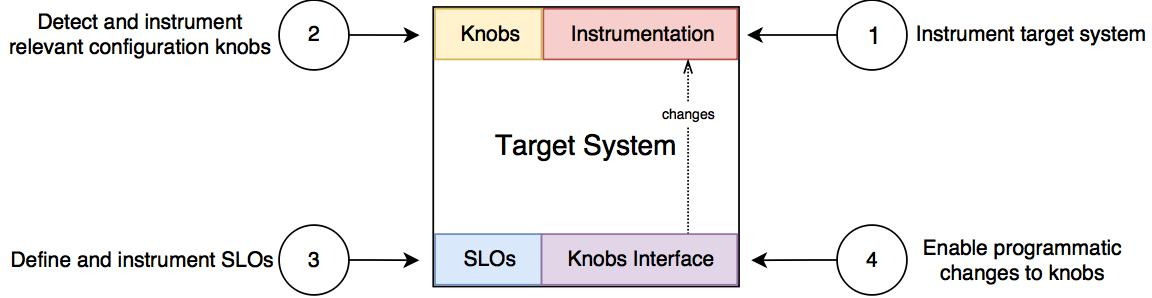
\includegraphics[width=\textwidth]{images/finch_user_perspective.jpg}
  \caption{\projectname{}'s approach from a user perspective. The four necessary steps to change the target system into a self-adaptive system}
  \label{fig:finch1}
\end{figure*}

\subsection{\projectname{} as a self-adaptation enabler}

In terms of self-adaptive systems, \projectname{} follows a centralized and top-down approach. According to the self-adaptive community, a centralized and top-down self-adaptive system operates with the guidance of a central controller, assesses its own behavior in the current surroundings, and adapts itself if the monitoring and analysis warrants it \cite{brun_engineering_2009}.

The main design goal in \projectname{} is to allow its users to inject feedback loops---based on the classic MAPE-K loop---through its API. As discussed by Y. Brun et al, to reason about uncertainty effectively, we need to elevate feedback loops to be visible and first class \cite{brun_engineering_2009}. However, rather than hard wiring the self-adaptation mechanisms inside the target system, \projectname{} keeps it loosely-coupled; the target system and \projectname{} work together to collect data about target system's environment and states, then \projectname{} store this knowledge for future reference and models training, with learned models ready to make predictions, \projectname{} watches and analyze event data and, based on its internal feedback loop, spits executions plans that aim to optimize the target system, this adaptation will lead to more event data that will be continuously stored and analyzed, where the cycle repeats.


% TODO: add some more context on "challenges ahead" in Y. Brun's paper. With Finch, we are tackling HCI, reengineering, and middleware components of his defined challenges

\subsection{System's heuristics and configuration as a learning problem}

A learning problem can be simply put as a set of observations comprised of input data and output data and some unknown relationship between the two, and the goal of a learning system is to learn a generalized mapping between input and output data such that predictions can be made for new instances drawn from the domain where the output variable is unknown.

The main hypothesis behind \projectname{} is that if we can model the configuration scheme or the heuristics of a system as a learning problem, then we can learn a model that can find patterns between the system's observations and the system's knobs---configuration knobs or the values used in heuristics that control the system's behaviors---enabling the system to predict the best set of knobs for a given specific observed scenario.

Because machine learning is about learning to predict a certain behavior in the future based on what was experienced in the past, an important step when modelling a problem as a learning problem is the choice of observations used to train the system.

In this context, observations could be anything that relates to the system's behavior, performance, inputs, and outputs. For instance: throughput, requests per second, latencies, and machine's resources usage---CPU and memory.

In \projectname{}'s case, it is important to give the necessary means to collect the best possible set of observations from the system and its environment. Thus, to model the system's heuristics and configuration as learning problem, \projectname{} assumes a system properly instrumented.

\subsection{Learnable patterns in systems context}

\subsubsection{System instrumentation}

The first step in our approach is to observe the system's behavior and context, this is an important technique to understand how a running system behaves; by having data that tells us how a system behaves under the combination of different workloads and different configuration knobs, we can see that interesting patterns emerge from this data.

Software instrumentation refers to pieces of code inserted in some parts of the system's codebase to record its context, for instance: the values of function parameters, latencies, and time to execute a certain block of code. The purpose of these pieces of code is to help measuring performance, debugging, finding bottlenecks, and similar tasks.

Luckily, the software industry has been enforcing system instrumentation by providing many solutions for software instrumentation and monitoring such as Dtrace \cite{cantrill_dynamic_2004}, Prometheus \cite{Prometheus}, Nagios \cite{Nagios}, and Datadog \cite{Datadog}.

Instrumentation is heavily used in industry also to detect Service Level Objectives (SLOs) violation and to perform resource management---two tasks that are crucial to \projectname{}.

Under \projectname{}'s layers all monitoring is performed using Prometheus. Prometheus is a pull-based monitoring tool and time-series database. A normal concern is: what is the overhead incurred by a pull-based monitoring tool? The answer to this question is straightforward: the overhead is negligible. Unlike monitoring tools like Nagios, which frequently executes check scripts, it only collects time series data from a set of instrumented targets over the network. For each target, the Prometheus server simply fetches the current state of all metrics of that target over HTTP and has no other execution overhead that would be pull-related.

Another reason why Prometheus overhead is low is that Prometheus is not an event-based system, it works by regularly collecting aggregated time series data that represents the current state of a given set of metrics, not the underlying events that led to the generation of those metrics. Thus, it does not send a message to Prometheus server for each request as it is handled, it simply count up those requests in memory---causing no monitoring overhead or traffic---then Prometheus pulls this data every few configurable seconds, returning the current counter value and its timestamp.

In this first step, what we ask from the users is to choose parts of their systems to instrument, more specifically, instrument parts that are closely related to performance and resource usage. What has showed to work for us---and for many practitioners in industry-- is to instrument: CPU usage, CPU idleness, memory usage, I/O writes per second, I/O reads per second, workload---it can be, for instance, requests per second---and latencies of desired services, for instance: the latency of each web service endpoint.

\subsubsection{Performance percentages and percentiles over average}

A common mistake both in industry and in the research community is measuring performance---specially latency or response time---using averages. Averages hide outliers and it is usually very skewed. To better illustrate this problem, consider having 100 requests per minute to your target system, if 80 of these requests take 200ms, which is relatively fast, and 20 of these requests take 10000ms, or 10 seconds, your average is $2.1$ seconds, which is an acceptable latency. However, it hides the fact that $20\%$ of these requests are taking an unacceptable amount of time to be served.

Rather than averaging performance metrics, \projectname{} takes three more reliable approaches to measure performance metrics:

\begin{itemize}
  \item Percentiles, such as 99th and 90th percentiles , in order to capture and understand outliers. This way we can understand upper bounds and uncover more silent bugs.
  \item Agreements on a percentage of requests being served under an agreed threshold. For example, an agreement could be: \textit{$95\%$ of the POST requests to endpoint $A$ will be served under 200ms}. This is a good strategy because rather than focusing on averaging---which is not reliable---we focus on serving well a big portion of the requests. This synergizes well with histograms and buckets.
  \item APDEX \cite{Apdex} as an extension on agreements.
\end{itemize}

APDEX is an industry standard that gives a score of satisfaction based on the latency or response time of requests. It is calculated by: $APDEX_T = \frac{S + \frac{T}{2}}{R}$. Where $T$ is a selected threshold, $S$ is the number of satisfied requests, or requests that take less than $T$ to be served, $T$ is the tolerated requests, or requests that take between $T$ and $T*4$ to be served, and $R$ is the total number of requests. A request is considered frustrated if it takes more than $T*4$ to be served.

To compare APDEX to averaging latencies, think of two scenarios:

\begin{itemize}
  \item $60\%$ of the requests take $200ms$, $20\%$ of the requests take $10ms$, and $20\%$ of the requests take 10 seconds. The average of latencies in this case is $2.1s$, which gives you a false sense of confidence. The $APDEX_{2s}$ is $80\%$, which is considered low.
  \item 1 request takes 5 minutes, 10 requests take 200ms. Here we have a case of anomalous latency. The average is 27 seconds, which is very high, whereas $APDEX_{2s}$ is $91\%$, telling us that, given our selected threshold, the situation is not bad, rather, it was just an anomalous case.
  
\end{itemize}

\projectname{} uses APDEX agreements and 99th and 90th percentiles as features and targets when training the predictions models.


\subsubsection{Configuration knobs instrumentation}

Now that we have data points that describe the performance and behavior of our system, we have to capture the current state of the configuration knobs; it can range from a variety of configurations, and it is highly dependent on the kind of system you are dealing with. Here we define a configuration knob as a property, parameter, or variable that holds a value that controls a certain aspect of a system or algorithm.

\subsubsection{Defining Service Level Agreements}

Having collected the instrumented data---data that represents the snapshot of both the configuration knobs and the performance at a given time---we have to point which of these instrumented data points are under service level agreements. Here we call these features Service Level Indicators (SLIs), they are a subset of the set of instrumented metrics that must satisfy a desired objetive, the SLA. 

For instance, given that we instrumented the latency of the endpoint $A$ of our web service, it is agreed that $95\%$ of the requests to this endpoint should have latency below $200ms$. This is properly captured by \projectname{}'s API.

% TODO: show formal language to capture this


\subsubsection{Resulting dataset}

We have collected four sets of features: metrics related to the system's context---performance and behavior metrics---configuration knobs, the workload, and service level indicators that must satisfy their objectives. The goal for the collection of this data is to build a dataset that will be used later to train models that will be used to make prediction based on these three sets of features, and the models will be trained to answer the following question: \textit{given a workload---e.g requests per seconds--- and the performance metrics of the system serving these requests, what is the optimal set of configuration knobs that will prevent service level objective violations?}

The dataset is constructed in such a way that each row describes the context of the system---workload, metrics, SLIS, and configuration knobs---at a given time captured by a timestamp.

The following matrix summarizes how the dataset is organized:

\setlength{\arraycolsep}{1pt}
\renewcommand\arraystretch{1.0}
\setcounter{MaxMatrixCols}{20}
$$
\begin{vmatrix}
  t_1 & W_1 & M_{1_1} & M_{2_1} & \dots & M_{i_1} & k_{1_1} & k_{2_1} & \dots & k_{t_1} & SLI_{1_1} & SLI_{2_1} & \dots & SLI_{\delta_1}\\
  t_2 & W_2 & M_{1_2} & M_{2_2} & \dots & M_{i_2} & k_{1_2} & k_{2_2} & \dots & k_{t_2} & SLI_{1_2} & SLI_{2_2} & \dots & SLI_{\delta_2}\\
  \vdots & \vdots & \vdots & \vdots & \ddots & \vdots & \vdots & \vdots & \ddots & \vdots & \vdots & \vdots & \ddots & \vdots \\
  t_n & W_n & M_{1_n} & M_{2_n} & \dots & M_{i_n} & k_{1_n} & k_{2_n} & \dots & k_{t_n} & SLI_{1_n} & SLI_{2_n} & \dots & SLI_{\delta_n}\\
\end{vmatrix}
$$

Where:

\begin{enumerate}
  \item $n$ is the number of collected samples
  \item $t_{\phi}$ is the timestamp of the $\phi-th$ example
  \item $M_{j_\phi}$ is the $j-th$ instrumented metric in timestamp $t_{\phi}$. $j$ ranges from $1$ to $i$, the last instrumented metric.
  \item $k_{c_\phi}$ is the value in the $c-th$ configuration knob in timestamp $t_{\phi}$. $c$ ranges from $1$ to $t$, the last collected configuration knob.
  \item $SLI_{o_\phi}$ is the $o-th$ service level indicator in the timestamp $t_{\phi}$---which is one of the instrumented metrics that was set to be an SLI. $o$ ranges from $1$ to $\delta$, the last collected SLI.
\end{enumerate}

This dataset should capture the context of a system with respect to workload, instrumented metrics, and the values in configuration knobs.  

\subsection{Machine learning architecture}

Given the previously defined dataset, \projectname{} trains many different models, each one targeting a different task. We have 2 ML pipelines: training the models, which also involves cross validating each model in isolation, and validating the prediction workflow: the workflow that triggers the interaction between the many models.

\subsubsection{Training the models}

There are two main classes of learned models:

\begin{enumerate}
  \item SLI models: these models predict, given the system's context, knobs values included, the SLI value. For instance, given the context, it outputs the latency of a certain endpoint. We will train a model for each collected SLI.
  \item Knob models: these models predict, given the system's context, other knobs \textit{not} included, one SLI $s$ included, and others SLIs that are not $s$ excluded, the optimal knob value. For instance, it outputs the optimal knob $k$ to achieve a certain latency $x$. We will train a model for each combination of SLI and knob collected.
\end{enumerate}

The training of the different models consists of slicing the original dataset to fit the models' needs. For instance, when we want to predict the latency of endpoint $A$, we must say that latency $A$ is the target, or $y$, of the model, and the corpus, or $X$, is the rest of the dataset \textit{minus} the latency $A$ column. Then we train the model passing this specific $X$ and $y$.

The algorithms \ref{alg:TrainSLIModels} and \ref{alg:TrainKnobModels} show with more details the process of training the models.
\SetInd{0.75em}{0.1em}
\begin{algorithm}
  \SetAlgoNoLine
  \caption{Trains a model for each SLI and return a list of models}\label{alg:TrainSLIModels}
  \SetKwInOut{Input}{inputs}
  \SetKwInOut{Output}{output}
  \SetKwProg{TrainSLIModels}{TrainSLIModels}{}{}

  \TrainSLIModels{$(Dataset)$}{
    \Input{A dataset that contains the system's context}
    \Output{$n$ SLI models, where $n$ is the number of collected SLIs}
    $models \gets []$ \;
    \ForEach{SLI $S \in Dataset$}{%
      $y \gets Dataset[S]$\;
      $X \gets Dataset \setminus Dataset[S]$\;
      $regressor \gets learning\_algorithm(...)$\; 
      $score \gets Cross\_validation(regressor, X, y$)\;
      \If{($score \geq 70\%$)}{%
        $models[S] \gets regressor.fit(X,y)$\;
      }
    }
    \KwRet{models}\;
  }
\end{algorithm}

Note that before training the final models, we cross validate the model with multiple---currently 100---splits of the dataset and performing the cross validation with 80/20 ratio: train with 80\% of the dataset, test with 20\% of the dataset, 100 times. This way we prevent cases of overfitting the model to the data.

\begin{algorithm}
  \SetAlgoNoLine
  \caption{Trains a model for each Knob x SLI combination and return a 2D array containing the models}\label{alg:TrainKnobModels}
  \SetKwInOut{Input}{inputs}
  \SetKwInOut{Output}{output}
  \SetKwProg{TrainKnobModels}{TrainKnobModels}{}{}

  \TrainKnobModels{$(Dataset)$}{
    \Input{A dataset that contains the system's context}
    \Output{$i *j$ $SLI \Rightarrow Knob$ models, where $i$ is the number of collected SLIs and $j$ is the number of collected knobs}
    $models \gets []$ \;
    \ForEach{SLI $S \in Dataset$}{%
      \ForEach{Knob $K \in Dataset$}{%
        $y \gets Dataset[K]$\;
        $X \gets Dataset \setminus Dataset[Knobs] \land Dataset[SLIs \neq S]$\;
        $regressor \gets learning\_algorithm(...)$\; 
        $score \gets Cross\_validation(regressor, X, y$)\;
        \If{($score \geq 70\%$)}{%
          $models[S, K] \gets regressor.fit(X,y)$\;
        }
      }    
    }
    \KwRet{models}\;
  }
\end{algorithm}

\subsubsection{Validating the prediction workflow}

The cross validation in algorithms \ref{alg:TrainSLIModels} and \ref{alg:TrainKnobModels} can only validate the accuracy of the each model in isolation. This is not enough to tell if the prediction workflow will work properly. For instance, one of our goals is to predict the best set of configuration knobs for a set of violated SLOs, so that after executing the adaptation plan, their respective SLIs will improve, preventing the SLO to be violated.

To achieve this level of validation, we perform bidirectional predictions: we grab a sample from the dataset that contains many SLO violations, predict the optimal knobs that could prevent the violations, then, using the predicted knobs, we predict the SLIs and see if it indeed improved in comparison to the original SLIs from the bad sample. Algorithm \ref{alg:ValidatePredictionWorkflow} shows with more details how this procedure works. 

\begin{algorithm}
  \SetAlgoNoLine
  \caption{Validates the prediction workflow by making bidirectional predictions. First we predict the best set of knobs given a bad scenario, then we predict the SLIs considering the predicted set of knobs}\label{alg:ValidatePredictionWorkflow}
  \SetKwInOut{Input}{inputs}
  \SetKwInOut{Output}{output}
  \SetKwProg{ValidatePredictionWorkflow}{ValidatePredictionWorkflow}{}{}

  \ValidatePredictionWorkflow{$(Dataset)$}{
    $test \gets Dataset[0]$ \;
    $X \gets Dataset[1:]$\;
    $SLI\_models = TrainSLIModels(X)$\;
    $knob\_models = TrainKnobModels(X)$\;
    $knob\_predictions \gets []$ \;
    \tcc{In this first foreach, we predict the optimal knob values for a sample with SLO violations}
    \ForEach{SLI $S \in Dataset$}{%
      $SLI\_test \gets test \setminus test[Knobs] \land test[SLIs \neq S]$\;
      \ForEach{Knob $K \in Dataset$}{%
        $pred \gets knob\_models[S,K].predict(SLI\_test)$
        $knob\_predictions[S, K] \gets pred$ \;
      }
    }
    $final\_knobs \gets$ most predicted set of knobs\;
    \tcc{Next we predict SLIs given the predicted set of knobs}
    $inverse\_test \gets test$ \;
    \ForEach{Knob $K \in Dataset$}{%
      $inverse\_test[K] \gets final\_knobs[K]$ \;
    }
    \ForEach{SLI $S \in Dataset$}{%
      $knob\_test \gets inverse\_test \setminus inverse\_test[S]$ \;
      Modify each remaining SLI value in $knob\_test$ to a value below its SLO \;
      $predicted\_sli \gets SLI\_models[S].predict(knob\_test)$ \;
      Validate that $predicted\_sli$ is below its SLO \;
    }
  }
\end{algorithm}


\subsection{Control-theoretic approach to self-adaptation}

Here we talk first about the architecture with regards to MAPE-k and how we generate adaptation plans. Then we talk about creating adaptation plans for future workload, by predicting the workload using time-series data.

\projectname{} offers a way to separate three main components in a traditional self-adaptive architecture: the monitoring process, the adaptation controller, and the management of control objectives (adaptation goals).

\subsubsection{Ahead-of-time adaptation}

As we showed before, the dataset contains the timestamp for each sample, meaning that we can take advantage of time-series analysis techniques to predict, given a certain time in the future, what will be the workload. Having the future workload in hands, we can use this data point to predict, like we did in the previous section, the best set of knobs based on the predicted SLIs.

The key trick is that this plan for the optimal set of knobs will not be immediately carried out---the time for this adaptation has not come yet. It will, however, be stored in a table that contains all scheduled plans, and an observer will be watching this table and carrying out the plans a few minutes before the prediction for a given workload.

Should it fail to predict the correct workload, it will, once again, predict the set of optimal knobs for the current workload and immediately carry out the plan.

This procedure will create adaptation plans for a short time window, executing adaptations before they are needed, thus, before a violation occurs.


\subsubsection{Online training}

Here we talk about the constant retraining of the models, since we will have data coming in all the data, so lots of corrections to be made.

\subsection{Propagating adaptation plans}

\section{Architecture and implementation}

\begin{figure*}[t]
  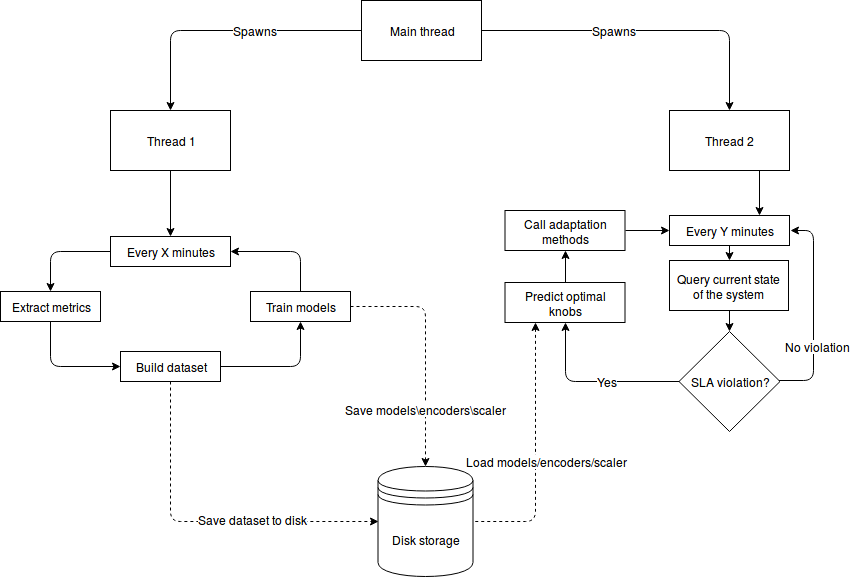
\includegraphics[scale=0.5]{images/FinchArchitecture.png}
  \caption{\projectname{}'s workflow architecture}
  \label{fig:finch2}
\end{figure*}

\projectname{}'s runtime spawns two main lightweight threads, which in Go (commonly referred as Golang) is called Goroutine. These two Goroutines are two observer threads. The first one is responsible for periodically building the dataset. It will, every $X$ minutes, where $X$ is configurable by the user, extract all collected metrics from Prometheus through its HTTP API, parse this data, and save the dataset. Then, it calls the machine learning component to train the models using this dataset, all models, scaler, and encoders---necessary components to make predictions---are persisted on disk.

The second Goroutine is responsible for monitoring the current state of the system by querying Prometheus every short period of time, and checking the APDEX score. Upon violation of an SLA, it calls the machine learning component, uses the most recently trained models to predict the best optimal knobs, then call each respective adaptation method responsible for changing that knob in the target system.

All infrastructure and main components of \projectname{} was built using Golang, due to its excellent performance and ease to build distributed and concurrent systems. However, Python was used to handle the machine learning components for its simplicity to quickly prototype and build mathematical models and experiments.

The interoperability test between Golang and Python was done by giving \projectname{}'s main components control over the machine learning component (written in Python). Because the machine learning component exposes a simple API, the main components use this API through executing bash commands. For instance:

\begin{lstlisting}
func predictOptimalKnobs(){
  cmd := Exec.command("python", "-c", "FinchML.predict_optimal_knobs")
  out, err := cmd.CombinedOutput()
  // out holds the optimal knobs
}
\end{lstlisting}

% TALK about that "propagation" effect or something like it.

\subsection{Adaptation methods}


\section{Evaluation}

To guide and evaluate our work, four research questions are used:

\begin{itemize}
  \item \textbf{RQ1:} Can self-adaptation by learned models lead to more stable and faster software systems, reducing the need to manually configure and tune?
  \item \textbf{RQ2:} How much instrumentation, SLO mapping, and configuration mapping is required to integrate the tool in a system?
  \item \textbf{RQ3:} How much performance overhead is incurred by using this tool?
  \item \textbf{RQ4:} What metrics and features have more impact on the tool's performance?
\end{itemize}

In the next subsection we discuss the setup for the experiment of the tool and techniques previously discussed.

\subsection{Experiment}

To evaluate the tool and the techniques here discussed, we developed a simple web service as the target system of \projectname{}. Although simple, this web service capture most commonly seen complexities, here is a brief description of it:

\begin{itemize}
  \item It consists of the backend component that holds all the core logic of the application.
  \item The application's services are exposed through many HTTP endpoints that follow a REST API approach. In our scenario, these endpoints are subject to a set of Service Level Agreements measured using APDEX. For instance, \textit{endpoint\_A\_POST} is a HTTP POST endpoint for the service $A$, and $X\%$ of all requests to it should not take more than $X ms$ to respond.
  \item This backend is containerized with Docker.
  \item Another Docker container holds a Postgres database used by the application.
  \item At last, another Docker container holds \projectname{} itself, including the vendors' tools used by it---Prometheus, for instance.
\end{itemize}

The reason why we had to develop our own target system, this web service, is that we needed a production-like web service exposed through a REST API. Since these types of systems are in fact a product, it is very hard to find these as open source, and the ones that you find are usually a simple proof of concept of a tool, for example: a web framework, with very few endpoints and simple business logic, which is not realistic enough to test \projectname{}.

\subsubsection{Initial training phase with workload simulation}

% Not sure if this subsection should go here or implementation details

\projectname{} starts making accurate and useful predictions after we have a dataset of reasonable size. In other words, the user must leave \projectname{} running for a while so that it can learn patterns in the target system and its workload. For that to happen in our experiment, we needed workload in our target system, however, since this is not a system in production, we needed to simulate a realistic workload with fluctuations (high and low workloads depending on day and time) and realistic and expected calls to the service's API based on use cases, for instance: a user could browse some shopping items, add them to the shopping card, go back and forth adding and removing shopping items, then she would go to the checkout page, and finalize the shopping session.

We created a workload simulation to mimic these use cases.

\subsubsection{Initial experiment with artificially generated knobs}

This first experiment intended to answer the following question: \emph{Can \projectname{} infer the optimal set of configuration knobs without being explicitly programmed to do so?}

To validate and answer this initial question, we needed not to focus on implementation details of the actual configuration changing, for example, gracefully handling Docker's containers and Postgresql restarts.

To achieve this, we created a script that randomly (and temporarily) generates blocking points in the target system, these blocking points block the flow in the code for either $B_i$ milliseconds or $\frac{1}{B_i}$ milliseconds for each blocking point $B \in 1 \dots i$. These $B_i$ values are now our configuration knobs that affect the performance of the target system. Thus, if \projectname{} can perform its workflow---monitor, analyze, predict, and execute the adaptation plan---and correctly configure the knobs in such a way that the performance will be optimal, again, without being explicitly programmed for this task, then we validate the architecture of \projectname{} is achieving its goals and that predicting actual configuration knobs is a matter of dataset quality, and thus, time to learn correctly.

We ran 3 different sets of artificially generated knobs and studied \projectname{} performance on them. (Here we show this data)

% The goal of this subsub is to motivate the use of the tool and techniques. We must show that default and static configurations cannot serve different scenarios
\subsubsection{The challenging task of configuring a Postgres database}

It is known that, because of the fact that Postgres contains a very big set of configurations knobs, it is a challenging task to adapt Postgres to different scenarios. For instance, for a certain type of query, properly configuring Postgres' \textit{work\_memory} variable can drastically improve its performance. There are many cases like this one, however, it would not be productive to discusss each one of them.

Postgres $9.4$ was used, and the configuration knobs considered were:

\begin{itemize}
  \item Shared buffers
  \item Effective cache size
  \item Work memory
  \item Write ahead log (WAL) buffers
  \item Checkpoint completion target
  \item Maintenance work memory
  \item Checkpoint segmnets
  \item Default statistics target
  \item Random page cost
\end{itemize}

In order to show that the Postgres default configuration is not the optimal one, we ran a workload simulation, which is similar to HTTP load testers, but instead of stressing a single endpoint with a very large number of requests per second, this workload simulation simulates different user workflows with varying intensities. For instance, 200 requests per second calling different sequences of endpoints: call endpoint $A$, wait for response, call $B$, wait response, and so on, until it completes a workflow that would be common for a user of this service. 

We ran the simulation---which tested the web application, and not the Postgres directly---for a certain period of time using two different sets of Postgres configuration knobs. By running this simulation we ended up with the dataset discussed in Section 3. The results confirmed both our beliefs and what is experienced in industry: The latencies of the endpoints were drastically affected by the different combinations of configuration knobs; different types of workflow and different intensities required different set of configurations in order to keep latency low, a non-optimal configuration for a given scenario could cause the violation of an SLO.

\iffalse
\begin{table}[]
  \centering
  \caption{My caption}
  \label{my-label}
  \begin{tabular}{llllllllll}
  Endpoint A(ms) & checkpoint\_completion\_target & checkpoint\_segments & default\_stat\_target & effective\_cache\_size & maintenance\_work\_mem & random\_page\_cost & shared\_buffers & wal\_buffers & work\_mem \\
  1846                                           & 0.1                                & 1                        & 30                              & 16                             & 8                              & 2                      & 16                      & 2                    & 512               \\
  1846                                           & 0.1                                & 1                        & 30                              & 16                             & 8                              & 2                      & 16                      & 2                    & 512               \\
  1846                                           & 0.1                                & 1                        & 30                              & 16                             & 8                              & 2                      & 16                      & 2                    & 512               \\
  119                                            & 0.5                                & 3                        & 100                             & 128                            & 16                             & 4                      & 128                     & 128                  & 1024              \\
  119                                            & 0.5                                & 3                        & 100                             & 128                            & 16                             & 4                      & 128                     & 128                  & 1024              \\
  119                                            & 0.5                                & 3                        & 100                             & 128                            & 16                             & 4                      & 128                     & 128                  & 1024             
  \end{tabular}
  \end{table}
\fi


\section{Discussion and future work}

\section{Conclusions}

%\end{document}  % This is where a 'short' article might terminate

\nocite{*}

%\begin{acks}

%\end{acks} 
% \begin{appendices}
\chapter{More on why using Go and Python}
Companies usually try to enforce homogeneous codebases, in other words: using a single language or the minimum possible number of languages, to both make it easier to maintain the codebase and to make it easier to hire engineers.

However, in this work we have decided to use 2 languages, the reason for that is that we believe we should use the right tools for a given job.

Machine learning tooling in Python is complete and backed by a strong community, the fact that Python is a dynamically typed languages makes total difference when performing data science experiments; we usually need to add and remove features as quickly as possible, and this can become very time demanding in a statically typed language with strict policies.

On the other hand, distributed and concurrent programming in Golang is as natural as the language itself can be; after all, these programming constructs are embedded in the language. Enforcing reliability in a system built in Golang is significantly easier than in systems built in Python.

And since \projectname{} needs to provide reliability, speed, and a fast way to experiment with machine learning using an arbitrary dataset, using Python for machine learning and wrapping its service and provide a solid infrastructure using Golang was the way to go.

The communication between these two components could be done using many common strategies such as exposing the machine learning service as a REST API, or using gRPC. However, that would introduce unnecessary complexities such as an HTTP and/or TCP layer, where all the communication between them is going to happen in the same machine---at least for now. Thus, exposing the machine learning component through a clean CLI-like API, and controlling it in Golang using Bash is the easiest and fastest way to achieve this communication.

% TODO: create image graph to illustrate this
\end{appendices}
\vfill % remove before submission
\pagebreak % remove before submission

\balance

\bibliographystyle{ACM-Reference-Format}
\bibliography{references} 

\end{document}
